\documentclass[a4paper, 12pt]{examen}

\begin{document}

%\modulo{Prog. multim. y de dispositivos moviles}
%\modulo{Planif. y adm. de redes}
%\modulo{Prog. de servicios y procesos}
\modulo{Lenguajes de marcas}


\pregunta{Elabora un fichero HTML que consiga lo que se muestra en la figura \ref{figurahtml}.  En este ejercicio se debe escribir todo el HTML, incluyendo cabecera,
cuerpo y elementos relevante para la estructura. }{3}

\begin{figure}[h]
    \caption{Resultado esperable en el ejercicio 1}
    \label{figura2}
    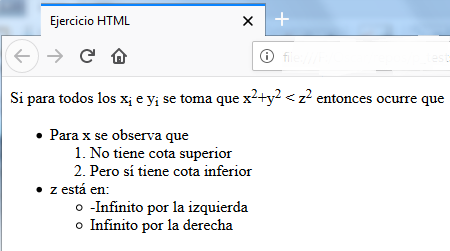
\includegraphics[scale=0.7]{foto_html.png}
\end{figure}
\break

\pregunta{ Elabora un fichero HTML que consiga exactamente
lo que se muestra en la figura \ref{figura2}. En este ejercicio solo hace falta escribir el HTML relevante, es decir, empezar por escribir la etiqueta {\tt table}}{  3.5 }
\begin{figure}[h]
    \caption{Resultado esperable en el ejercicio 2}
    \label{figura2}
    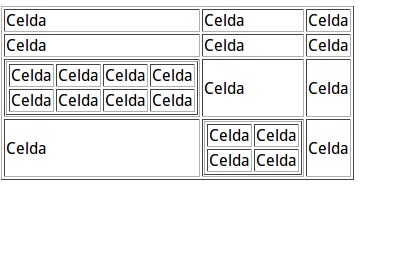
\includegraphics[scale=0.7]{foto_07.png}
\end{figure}
\break



\pregunta{ Elabora un fichero HTML que consiga exactamente
lo que se muestra en la figura \ref{figura1}. En este ejercicio solo hace falta escribir el HTML relevante,
en este caso solo a partir de la etiqueta {\tt table}
Ten en cuenta que:

\begin{itemize}



    \item{Hay un textarea que mide 4 filas y 52 columnas que lleva dentro el texto ``Utilice este cuadro para escribir''}

    \item{Hay un control para indicar la fecha.}

    \item{Hay un control para elegir el color.}

    \item{Contiene los siguientes checkboxes:checkbox con el name ``conector'' , value ``conectorusb'' y el texto ``USB'', checkbox con el name ``conector'' , value ``conectorparalelo'' y el texto ``Paralelo'', checkbox con el name ``conector'' , value ``conectorps2'' y el texto ``PS2''.}

    \item{Hay una lista desplegable con el name ``aula'' y con las siguientes opciones: opción ``A01'' con el value a01, opción ``A02'' con el value a02, opción ``A03'' con el value a03.}

    \item{Hay un control para elegir ficheros.}

    \item{Hay los siguientes cuadros de texto:cuadro de texto con el texto ``Nombre'' y el name nombre, cuadro de texto con el texto ``Apellidos'' y el name apellidos}

\end{itemize}

}{  3.5 }
\begin{figure}[h]
    \caption{Resultado esperable en el ejercicio del formulario.}
    \label{figura1}
    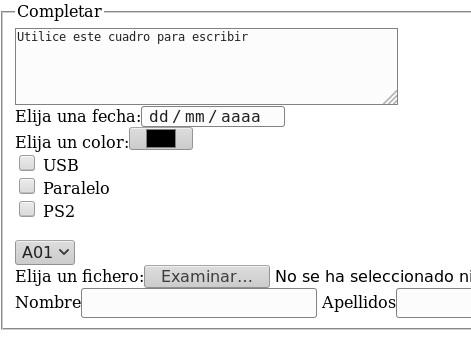
\includegraphics[scale=0.7]{foto_formulario_12.png}
\end{figure}


\end{document}
